\documentclass{article}%
\usepackage[T1]{fontenc}%
\usepackage[utf8]{inputenc}%
\usepackage{lmodern}%
\usepackage{textcomp}%
\usepackage{lastpage}%
\usepackage{geometry}%
\geometry{margin=1in}%
%
\usepackage{subcaption}%
\usepackage{amsmath}%
\usepackage{amssymb}%
\usepackage{booktabs}%
\usepackage{longtable}%
\usepackage{graphicx}%
\usepackage{float}%
\usepackage{caption}%
\usepackage{hyperref}%
\usepackage{listings}%
\usepackage{xcolor}%
\lstdefinestyle{mystyle}{backgroundcolor=\color{lightgray}, commentstyle=\color{green}, keywordstyle=\color{blue}, numberstyle=\tiny\color{gray}, stringstyle=\color{red}, basicstyle=\ttfamily\footnotesize, breakatwhitespace=false, breaklines=true, captionpos=b, keepspaces=true, numbers=left, numbersep=5pt, showspaces=false, showstringspaces=false, showtabs=false, tabsize=2}%
\lstset{style=mystyle}%
\title{CHE 565 {-}{-} Exam 2}%
\author{Soki Sem}%
\date{\today}%
%
\begin{document}%
\normalsize%
\setlength{\parindent}{0pt}%
\setlength{\parskip}{0.6em}%
\maketitle%
\section*{Problem 1}%
\label{sec:Problem1}%
\subsection*{A}%
\label{subsec:A}%
\begin{figure}[H]%
\centering%
\begin{subfigure}{0.45\textwidth}%
\centering%
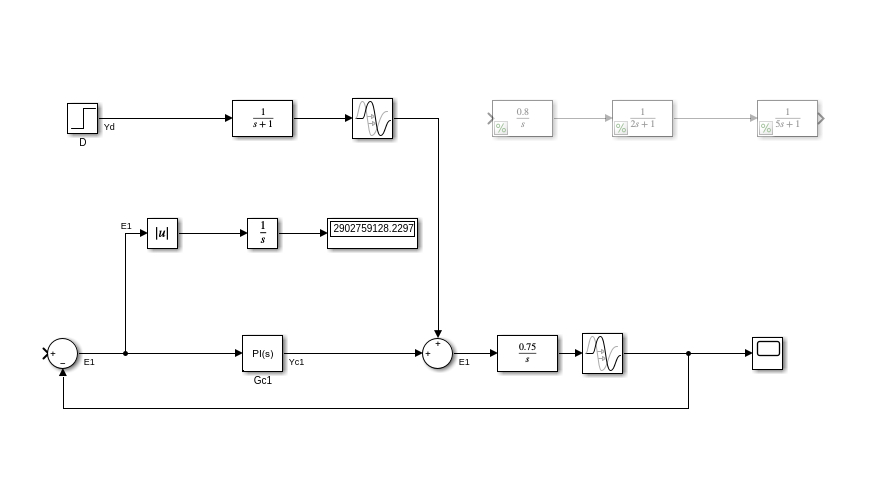
\includegraphics[width=\linewidth]{Exam2_block_diagram_disturbance.png}%
\subcaption{Disturbance Diagram}%
\end{subfigure}%
\begin{subfigure}{0.45\textwidth}%
\centering%

\includegraphics[width=\linewidth]{Exam2_block_diagram_setpoint.png}%
\subcaption{Setpoint Diagram}%
\end{subfigure}%
\caption{Block Diagram Control System}%
\end{figure}%
\begin{align*}%
\text{Process Transfer Function:} \frac{0.8}{s \left(2 s + 1\right) \left(5 s + 1\right)} \\%
\text{Modeled Process Transfer Function:} \frac{0.75 e^{- 4 s}}{s} \\%
\text{Disturbance Transfer Function:} \frac{e^{- s}}{s + 1}%
\end{align*}%
Using lambda tuning for PI control, we find the controller parameters as follows:%
\par%
\begin{align*}%
K' = \frac{K_p}{\tau_p},Kc = \frac{\tau_p}{K' (\lambda + \theta_d)^2} \\%
\tau_{I} = \tau_p \\%
\lambda = 8 \theta_d \\%
\tau_D = 0%
\end{align*}%
Where %
$\tau_p$%
= 1%
$\quad$%
$\theta_d$%
= 4%
$\quad$%
$K_p$%
= 0.75%
\par%
$K_c:$%
= 0.0700 %
$\tau_I:$%
= 68.0000 %
$\lambda:$%
= 32.0000 %
$\tau_D:$%
= 0.0000 %
$\quad$%
And an IAE of:%
$\quad$%
417965.4725%
$\quad$%
for the setpoint change and%
$\quad$%
123704.5080%
$\quad$%
for the disturbance.%
\par%
\begin{figure}[H]%
\centering%
\begin{subfigure}{0.45\textwidth}%
\centering%
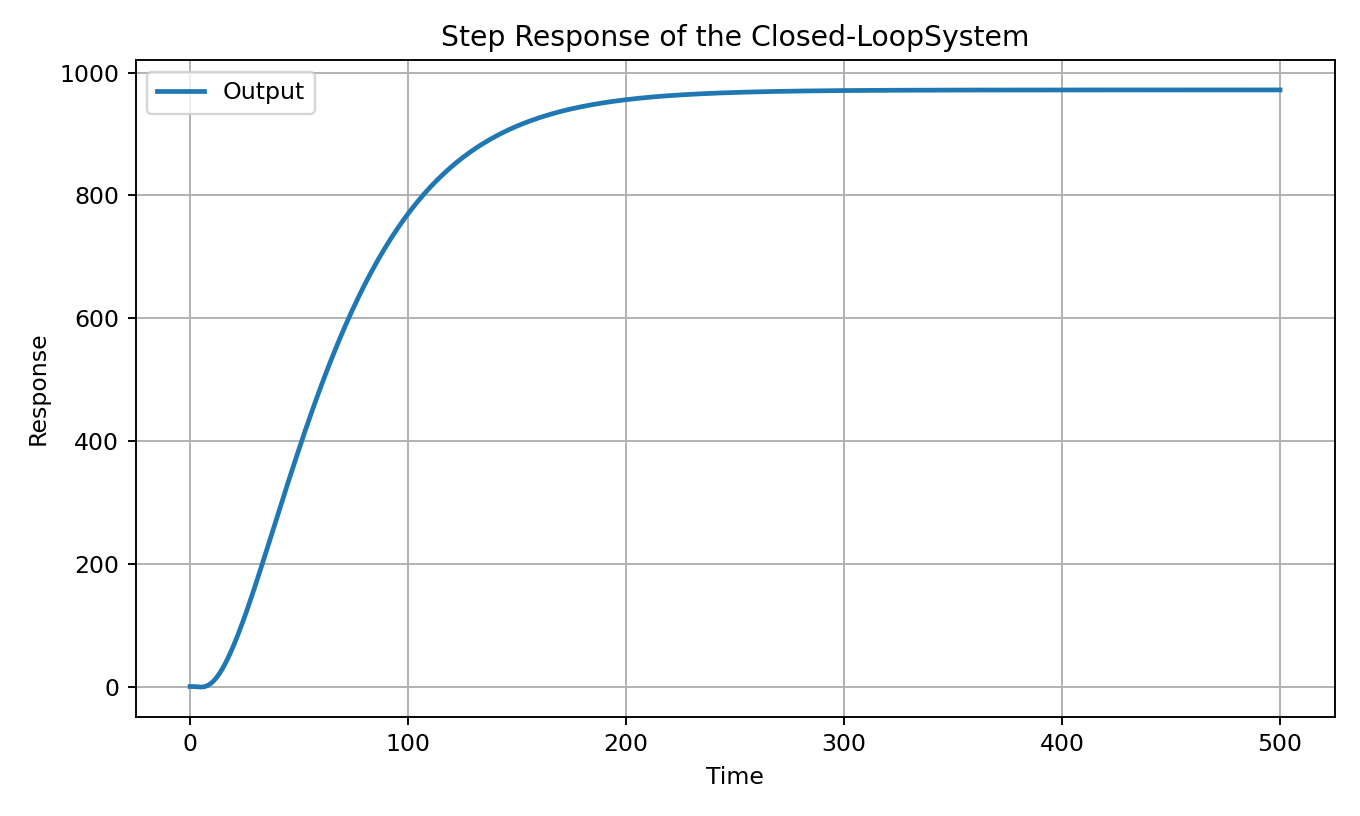
\includegraphics[width=\linewidth]{problem1_disturbance.png}%
\subcaption{Disturbance}%
\end{subfigure}%
\begin{subfigure}{0.45\textwidth}%
\centering%

\includegraphics[width=\linewidth]{problem1_setpoint.png}%
\subcaption{Setpoint Change}%
\end{subfigure}%
\caption{Closed{-}Loop Step Responses}%
\end{figure}

%
\end{document}